\section{Introduction}
The Introduction delivers the motivation for your paper. 
It explains \emph{why} you did the work you did. 
This is the primary function of the Introduction.
I have found a 5-point structure for Introductions to be particularly effective. (Here, I build on advice I received as
a Ph.D. student from Prof. Scott E. Hudson.)

\begin{itemize}
    \item State of the world…
    \item The big BUT...
    \item Therefore, we did...
    \item The key findings are...
    \item The contributions of this work are...
\end{itemize}

The state of the world is a description of issues in whatever \say{world} is relevant to your topic. 
Drawing on popular press can be effective here if recent news items or data from articles support your cause.

The big BUT is where a problem is introduced.
Or, similarly, a problem can be framed as an opportunity. 
Whether you are solving a problem or seizing an opportunity, motivate your work by connecting it to \emph{things that matter to people}.

One of the worst ways to motivate your work is using the \say{absence from the literature} argument. 
\say{Studies to date have
not …,} or \say{The literature is thus far silent on…,} or \say{Researchers have not yet examined how…} 
Such sentences are fine to add \emph{after} you have established a problem or opportunity worthy of pursuit in its own right. 
But as standalone motivational statements, absence-from-the-literature does not zing. 
Maybe the literature is silent on an issue
because that issue is not important.

After the big BUT, you will describe what you did, now in a bit more detail than in the Abstract. 
Devoting a paragraph to what you did is reasonable in the Introduction.

After saying what you did, you should offer the key results of what you did. 
What were the major findings? 
Whereas the Abstract might have devoted a sentence or two to key results, now you can devote a whole paragraph.

Finally, a good way to end your Introduction is by framing the contributions that your work makes. (See \say{Seven Research Contributions in HCI}\cite{wobbrock2012seven} for examples of different research contributions.) 
I often structure my contributions as a numbered list within a paragraph.
\say{The main contributions of this work are: (1) …; (2) …; (3) …}
(Most papers will have one to three contributions. 
Work that claims to have more than three contributions is often overstating how many contributions it makes.)

By structuring your Introduction with the 5-point outline, you succinctly motivate the work against a real problem or opportunity, and hook the reader by enticing them with the key results and contributions. 
They will want to know more.

Often, reviewers’ judgments about a piece are formed pretty quickly after reading the Introduction. 
If the Introduction reads poorly or is missing key aspects, that judgment can tilt negative very quickly.

Whatever expectations you set up in the Introduction, whatever research claims you make, you must deliver upon them in the rest of the paper. 
Over-claiming is a sure way to
get your paper rejected.

Do not make the main implication of your research that more research is needed. 
(It can be an implication, but not the main one, and certainly not the one called out at the end of the Introduction, Abstract, or Conclusion.) 
An Introduction (or Abstract or Conclusion) that ends with, “This work opens up new directions for further research into X” as its main answer to “so what?” is weak and uninspiring. 
What such a statement essentially means is that the chief benefit of your research is just more research. 
And apparently that research is left for others to do because, for some reason, you stopped short of doing it. 
Instead, make the main implication of your work that the problem or opportunity you set out to address is now at least somewhat addressed. 
\say{This work paves the way for more women to be better incorporated into software
development teams.} 
\say{This work opens up new directions in the development of assistive technology by using adaptive
user interfaces.} 
\say{This work lessens the challenges faced by single mothers as they try to incorporate educational technologies into their children’s lives.} 
The point is, the outcome of your research can’t just be more research, or why didn’t you do it and gain an actual solution to report?

In a 10-page paper, it is okay if the Introduction goes a bit onto the second page. 
In a 4-page paper, the Introduction should probably end somewhere on the first page.\footnote{April: Your final thesis report should range between 5 to 10 pages in length. It should not encompass every detail of your work but rather summarize and present it concisely.}

\begin{figure}
    \centering
    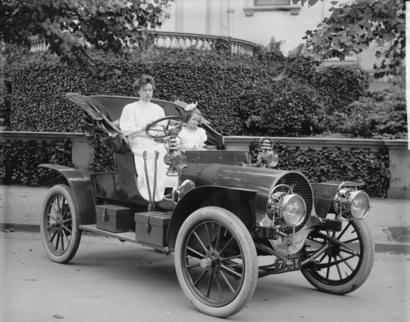
\includegraphics{figures/sample-franklin.png}
    \caption{Caption}
    \label{fig:enter-label}
\end{figure}